\section{Failures at Scale}
In this section we discuss how and why knowledge markets may fail at scale. We first empirically examine diseconomies of scale (Section 8.1), then analyze the effects of scale on market health (Section 8.2), and finally study user exchangeability under scale changes (Section 8.3).

\subsection{Diseconomies of Scale}
First, we examine disceconomies of scale---the ratio of answers to questions declining with the increase in number of users. The opposite of diseconomies is economies, when the ratio increases with the increase in number of users. The concept of diseconomies is important because the decrease in answer to question ratio implies the increase in gap between market supply (answer) and demand (question). In fact, if the ratio falls below 1.0, the gap becomes critical---guaranteeing there will be some questions with no answers. 
%We observe disceconomies of scale in most Stack Exchange markets.

\begin{figure}[hbt]
\vspace{-0.5\baselineskip}
\centering
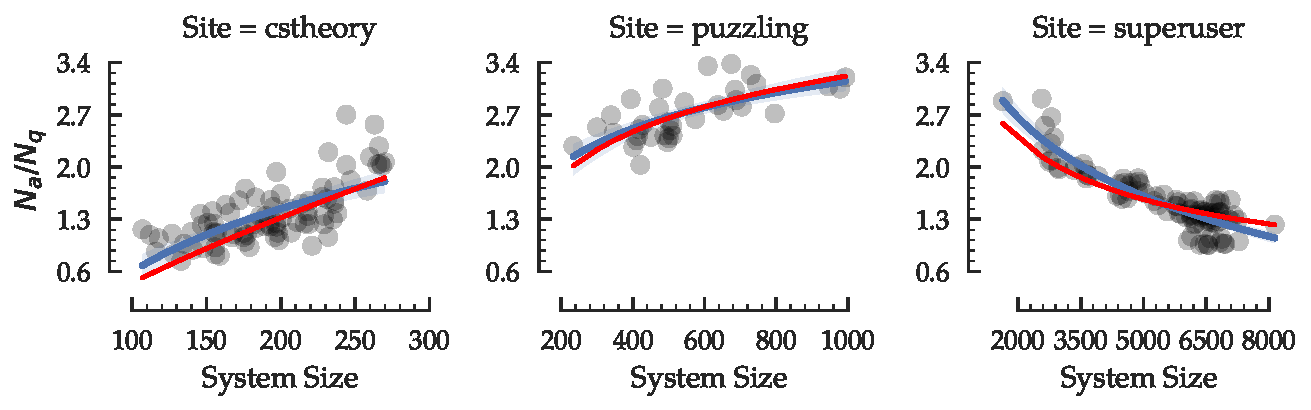
\includegraphics[scale=0.39]{Figures/Size_vs_Diseconomy.pdf}
\vspace{-2\baselineskip}
\caption{Diseconomies and economies of scale: the ratio of answers to questions decreasing (diseconomies) or increasing (economies) with the increase in number of users. 124 (out of 156) Stack Exchange markets exhibit diseconomies of scale. Examples: \texttt{superuser} (strong diseconomies), \texttt{puzzling} (weak economies), and \texttt{cstheory} (strong economies). }
\vspace{-\baselineskip}
\label{fig:diseconomy}
\end{figure}

In Figure~\ref{fig:diseconomy} we present the economies and diseconomies of scale in three Stack Exchange markets: \texttt{cstheory}, \texttt{puzzling} and \texttt{superuser}. We choose these examples to cover three cases: strong diseconomies, strong economies, and weak economies. Among the three markets, \texttt{superuser} shows strong diseconomies of scale: if the number of users increases by 1\%, then answer to question ratio declines by 0.95\%. The other two markets show economies of scale, where \texttt{cstheory} shows strong economies: if the number of users increases by 1\%, then answer to question ratio increases by 0.8\%; and \texttt{puzzling} shows weak economies: if the number of users increases by 1\%, then answer to question ratio increases by 0.2\%. Note that most markets, especially the ones with more than 500 monthly active participants, exhibit diseconomies of scale similar to \texttt{superuser}. Only five markets exhibit strong economies of scale in Stack Exchange: \texttt{cstheory}, \texttt{expressionengine}, \texttt{puzzling}, \texttt{ja\_stackoverflow}, and \texttt{softwareengineering}.

The Cobb-Douglas curves well fit the empirical trends of economies and diseconomies (as shown in Figure~\ref{fig:diseconomy}). We derive these curves by dividing the answer models by the corresponding question models, and subsequently developing curves that capture economies and diseconomies ($N_{a/q}$) as a function of number of users (system size). We get similar curves via log regression. Between the two model types, the Cobb-Douglas models provide better explanation.

The Cobb-Douglas models well explain the economies and disceconomies of scale. As per the models, the primary cause of disceconomies is the difference between the diminishing returns of questions and answers for user participation. In other words, in most market, for user input, the marginal question output is higher compared to marginal answer output, i.e., an average user is likely to ask more questions and provide few answers. This causes the ratio of answers to questions to decline with the increase in number of users. 

\subsection{Analyzing Health}
Next, we examine the disadvantage of scale through two health metrics--- $H_1:$ fraction of answered questions (questions with at least one answer); and $H_2:$ fraction of questions with accepted answer (questions for which asker marked an answer as accepted). $H_1$ and $H_2$ capture the true gap between market supply (answer) and demand (question). The increase in number of users may cause decline in $H_1$ and $H_2$, as both metrics are related to the ratio of answer to questions. In fact, if the ratio falls below 1.0, it guarantees the decline of both metrics. 

\begin{figure}[hbt]
\vspace{-0.5\baselineskip}
\centering
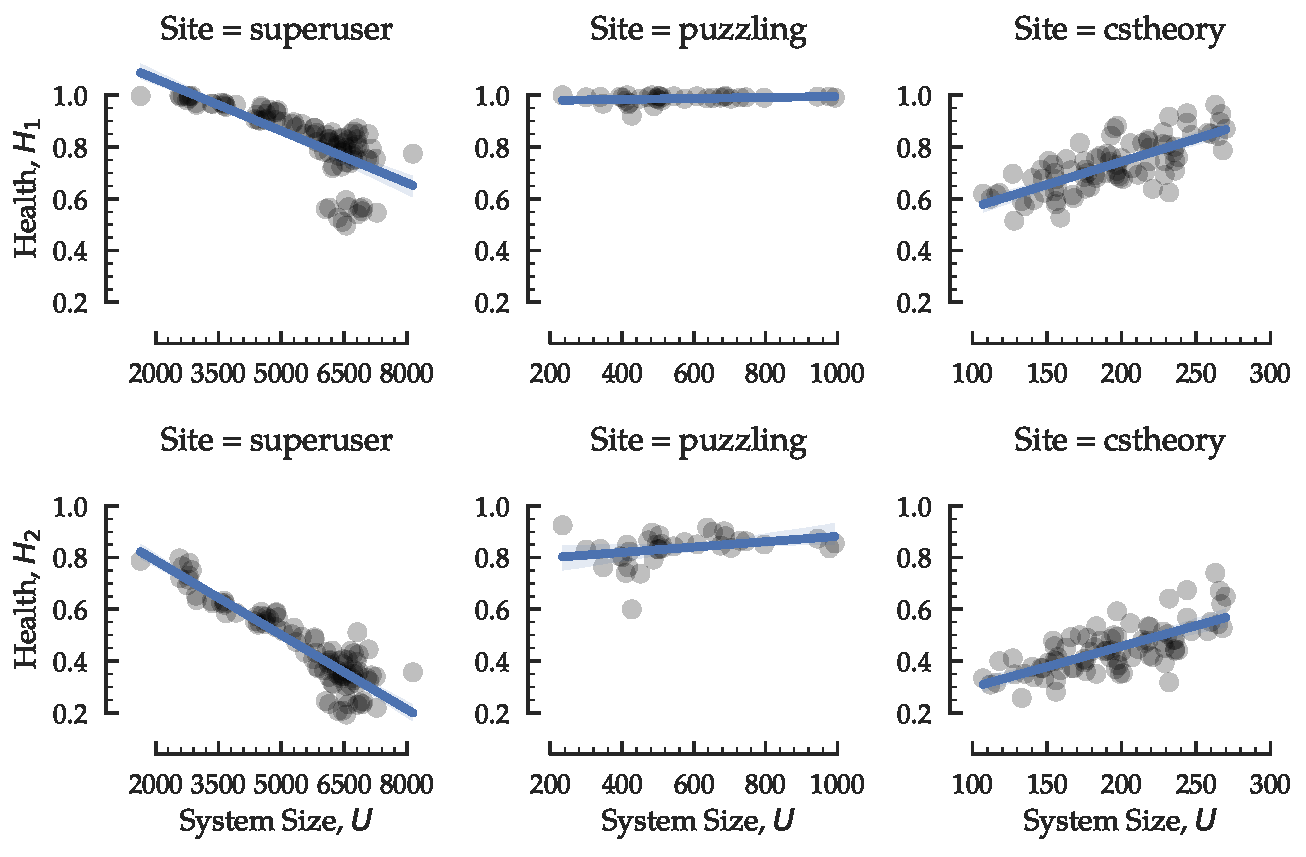
\includegraphics[scale=0.39]{Figures/Size_vs_Health.pdf}
\vspace{-2\baselineskip}
\caption{Health disadvantage and advantage of scale: the fraction of answered questions ($H_1$) and the fraction of questions with accepted answer ($H_2$) decreasing (disadvantage) or increasing (advantage) with the increase in number of users.141 (out of 156) markets exhibit disadvantage at scale. Examples: \texttt{superuser} (disadvantage), \texttt{puzzling} (neutral), and \texttt{cstheory} (advantage).}
\vspace{-\baselineskip}
\label{fig:health}
\end{figure}

In Figure~\ref{fig:health} we present the advantage and disadvantage of scale (through $H_1$ and $H_2$) for three Stack Exchange markets: \texttt{cstheory}, \texttt{puzzling} and \texttt{superuser}. We observe that the results are consistent with our analysis of economies and diseconomies---\texttt{cstheory} exhibit health advantage at scale, \texttt{puzzling} remains stable, whereas \texttt{superuser} exhibit disadvantage at scale. These three examples cover the possible health effects of scale in knowledge markets. 

%We cluster the markets based on model parameters and examine their health. In particular, we use kmeans clustering with silhouette analysis to determine two clusters. Figure x shows the clusters in a 3d space, reduced via Isomap reduction. Figure y shows the health summary for the two clusters. There exists a clear gap between the health of the two clusters. The first group is somewhat more robust to scale, whereas the second group is vulnerable at scale.

\subsection{Effects on Exchangeability}
Now, we empirically study the effects of scale on user exchangeability. By exchangeability, we specifically mean the gap between the top contributors and other participants in a knowledge market. Studying this gap is important because it can reveal if a market's success or failure depends on a small group of users.  

To empirically study user exchangeability, we define two metrics that reflect the gap between the top contributors and other participants in a knowledge market. The first metric $I_1$ is defined as the ratio of average contribution for top k\% users and bottom k\% users. For computing $I_1$, we measure the contribution of each user as the ratio ($n_{a/q}$) of number of answers provided by the user to the number of questions asked by the user. Notice that $I_1$ is a ratio based metric and we define user contribution to be consistent with this metric. The second metric $I_2$ is defined as the sum of two distance: (i) the distance between the contribution of top k\% users and average k\% users, and(ii) the distance between the contribution of average k\% users and bottom k\% users. For computing $I_2$, we measure the contribution of each user as a tuple ($n_a, n_q$), consisting of the number of answers ($n_a$) provided by the user and the number of questions asked by the user ($n_q$). Notice that $I_2$ is an interval based metric and we define user contribution to be consistent with this metric. While both metrics have certain limitations (e.g., does not account for other content types), these metrics allow us to comprehend user exchegeability in Stack Exchange.

\begin{figure}[hbt]
\vspace{-0.5\baselineskip}
\centering
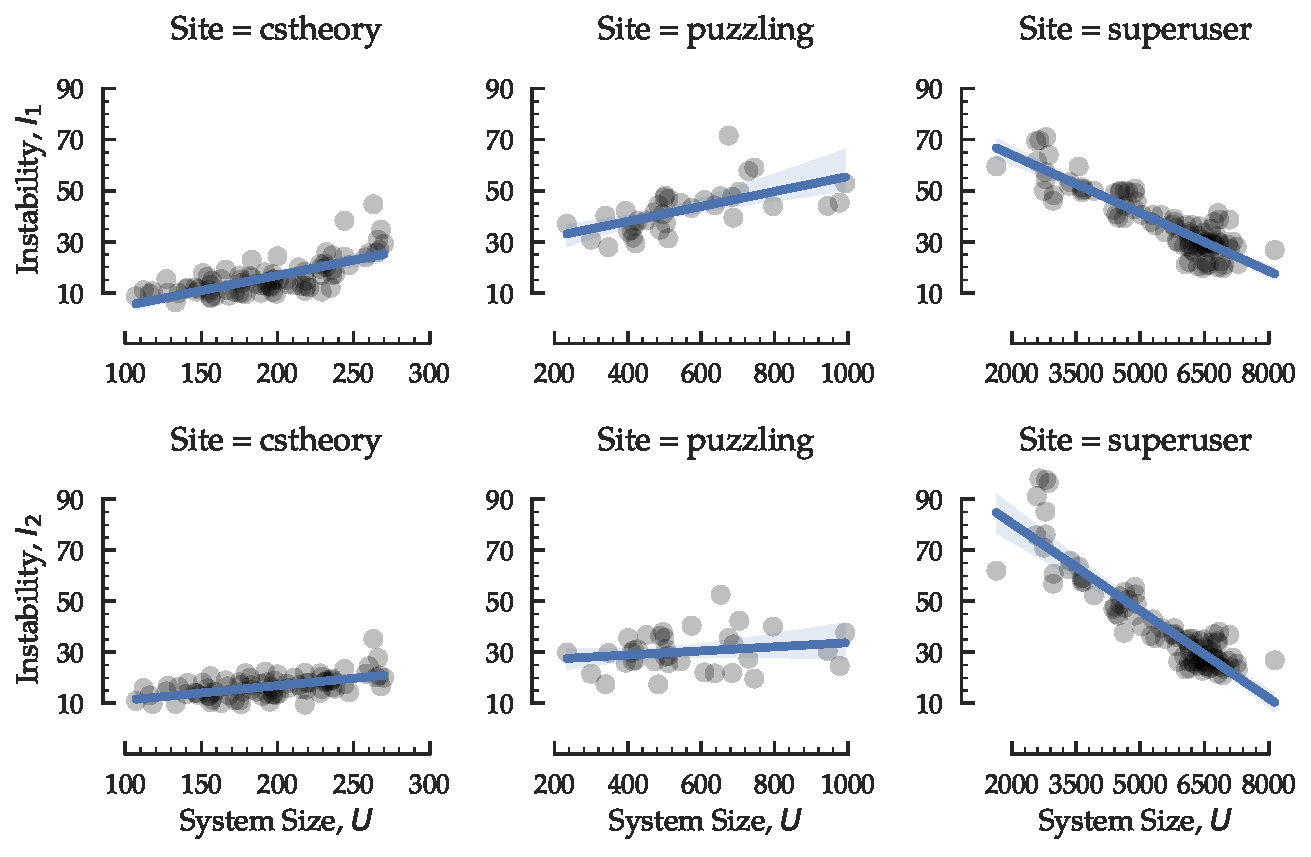
\includegraphics[scale=0.39]{Figures/Size_vs_Instability.pdf}
\vspace{-2\baselineskip}
\caption{User exchangeability under scale: the gap ($I_1$ or $I_2$) between the top contributors and other participants in a knowledge market decreasing or increasing with the increase in number of users. Most markets exhibit a large gap between the top contributors and other participants, i.e., participants are dissimilar. Examples: \texttt{superuser} (high dissimilarity), \texttt{puzzling} (moderate dissimilarity), and \texttt{cstheory} (low dissimilarity).}
\vspace{-\baselineskip}
\label{fig:stability}
\end{figure}

In Figure~\ref{fig:stability} we present the exchangeability of users under scale changes (through $I_1$ and $I_2$) for three Stack Exchange markets: \texttt{cstheory}, \texttt{puzzling} and \texttt{superuser}. Among the three markets, \texttt{superuser} exhibit the highest gap between top contributors and the other participants. However, as the number of participants increase, this gap decreases, i.e., the users become more exchangeable. In contrast, \texttt{cstheory} exhibit the lowest gap between top contributors and the other participants. However, as the number of participants increase, this gap increases, i.e., the users become less exchangeable.

